\documentclass[12pt, letterpaper]{report}
\usepackage[utf8]{inputenc}
\usepackage[T1]{fontenc}
\usepackage[a4paper,left=2cm,right=2cm,top=2cm,bottom=2cm]{geometry}
\usepackage{booktabs}
\usepackage[french]{babel}
\usepackage{libertine}
\usepackage[pdftex]{graphicx}
\usepackage{csquotes}
\usepackage{url}
\usepackage{hyperref}
\hypersetup{colorlinks=true,linkcolor=black}


\setlength{\parskip}{1em}
\setlength{\parindent}{0em}
\newcommand{\hsp}{\hspace{20pt}}
\newcommand{\HRule}{\rule{\linewidth}{0.5mm}}

\begin{document}
\begin{titlepage}
  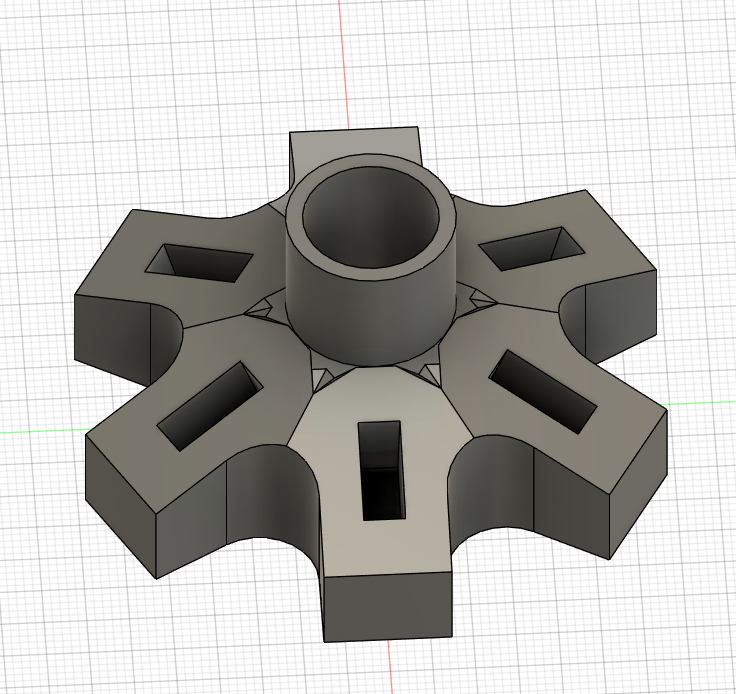
\includegraphics[scale=0.7]{IMG1.JPG}
  \begin{sffamily}
    \begin{center}


      \textsc{\LARGE Henallux - Institut d'enseignement supérieur de Namur}\[2cm]

        \textsc{\Large Laboratoire de sciences appliquées à l'informatique}\[1.5cm]

          \HRule \[0.4cm]
            \huge \bfseries {Laboratoire \#01 - Analyse de signaux \[0.4cm]}
              \HRule \[2cm]

                \begin{minipage}{0.4\textwidth}
                  \begin{flushleft} \large
                    Schoonjans \textsc{Ludovic}\
                    Vanderbeken  \textsc{Mathias}\
                    Dubois  \textsc{Aaron}\
                    Combette  \textsc{Nathan}\
                  \end{flushleft}
                \end{minipage}
                \begin{minipage}{0.4\textwidth}
                  \begin{flushright} \large
                    \emph{Professeur :} \textsc{Guillerme Duvillié}\
                    \emph{Groupe :} \textsc{Les coléoptères \du frigos}\
                  \end{flushright}
                \end{minipage}

                \vfill

                \large 18 Avril 2023
    \end{center}
  \end{sffamily}
\end{titlepage}

\renewcommand*\contentsname{Table des matières}
\tableofcontents

\chapter{Introduction}
L'objectif de cette étude est de comprendre le fonctionnement de la transmission d'un signal à travers les ports COMx (série) en utilisant la norme RS232. Pour cela, nous avons simulé l'envoi d'informations à travers ce port et redirigé le signal vers un oscilloscope pour analyser son fonctionnement. Le matériel utilisé comprend un oscilloscope, un multimètre, un boitier de visualisation RS232, un ordinateur équipé d'un port COM (série), un câble de liaison série et le programme PortComPC.
\chapter{Notions théoriques}
La norme RS232 est une norme d'échange de données utilisée pour la communication entre les ports COM, qui sont des ports série. La transmission des données se fait en commençant par un bit de départ (0 logique), suivi des données (de 5 à 9 bits en général), et enfin d'un ou plusieurs bit(s) de fin (1 logique). Les données sont transmises du Least Significant Bit (LSB) au Most Significant Bit (MSB). La norme RS232 utilise des tensions opposées pour représenter les bits logiques, avec un 1 logique correspondant à une tension négative et un 0 logique correspondant à une tension positive. L'ASCII est utilisé pour représenter les caractères alphanumériques en binaire. Le baud rate indique la vitesse de transfert de l'information à travers le câble série, exprimée en bits par seconde (bps).

\chapter{Manipulation}
\section{Connexion physique}
Le boitier de visualisation RS232 a été connecté à l'ordinateur via son port série (COM), et l'autre extrémité du câble série a été connectée à la fiche supérieure du boîtier RS232.
\section{Mesures et tests}
Les niveaux de tension aux bornes des douilles DTR et RTS ont été testés en utilisant le logiciel PortComPC. Les tensions mesurées pour les bits logiques 0 et 1 étaient respectivement d'environ -10.4 V et 10.57 V pour DTR, et -10.39 V et 10.58 V pour RTS.
\section{Analyse du signal}
L'oscilloscope a été connecté aux bornes "TX" pour analyser le code binaire envoyé par le logiciel. Le signal capturé correspondait au caractère "T" en ASCII (01010100), avec les particularités attendues selon le protocole RS232.
\section{Envoi et réception}
Le branchement a été modifié pour relier la borne TX à la RX, permettant ainsi de rediriger le signal vers l'oscilloscope et vers la fenêtre de réception du logiciel PortComPC. Les données envoyées étaient bien reçues convenablement.
\section{Analyse d'un message en détail}
Un message plus complet a été envoyé, représentant la valeur 521 en ASCII. L'oscilloscope a reçu le signal correspondant, qui a été décodé et vérifié avec succès.

\chapter{Conclusion}
La communication série, en utilisant la norme RS232, permet d'envoyer des informations sous forme de signal électrique à travers un câble série. Le récepteur peut ensuite traiter ces signaux pour reconstituer l'information originelle. Le protocole RS232 utilise un signal bas pour annoncer le début de l'envoi, suivi des données transmises du LSB au MSB, et se terminant par un bit de fin (1 logique).

Cette méthode de communication nécessite également l'établissement d'une horloge, qui indique la cadence à laquelle l'information est envoyée. Le "baud rate" est le nombre de bits transmis par seconde. Une cadence fréquente est de 9600 bps, et c'est celle que nous avons utilisée dans cette étude.

Bien que les ports série aient été en grande partie remplacés par des technologies plus modernes telles que l'USB, ils restent pratiques pour la communication entre deux machines, comme par exemple pour connecter des routeurs entre eux au sein d'un même sous-réseau. Les résultats de cette étude démontrent que la transmission d'informations à travers les ports COMx en utilisant la norme RS232 est un moyen fiable et efficace de communication entre dispositifs.
\chapter{Bibliographie}

$[Fig.2.1]$ {https://m.media-amazon.com/images/I/71xb7p6G5lL.\_SX522\_.jpg}

$[1]$ \textsc{Wikipédia}, \emph{Loi d'Ohm}, \newline
{https://fr.wikipedia.org/wiki/Loi\_d\%27Ohm},\quad consulté le 03/04/2023 à 14h43.
\smallskip

$[2]$ \textsc{Wikipédia}, \emph{Décibel}, \newline
{https://fr.wikipedia.org/wiki/Décibel},\quad consulté le 03/04/2023 à 14h02.
\smallskip

$[3]$ \textsc{Wikipédia}, \emph{Énergie électrique},\newline
{https://fr.wikipedia.org/wiki/Énergie\_électrique},\quad consulté le 03/04/2023 à 14h47.

\end{document}
